\section{Introduction}
\label{section:introduction}

Large language models (LLMs) such as GPT-4, Gemini, and Llama have
demonstrated exceptional capabilities across a variety of tasks,
ranging from natural language understanding to complex reasoning
\citep{achiam2023gpt,team2023gemini,dubey2024llama}. By virtue of
their massive parameter counts and rich training corpora, LLMs
have achieved human-level fluency and remarkable reasoning
capabilities across diverse domains. However, with scale also comes a
significant challenge: the propensity to memorize large parts of their
training data \citep{carlini2021extracting}. As model sizes grow, so
does the severity of memorization \citep{carlini2022quantifying,
biderman2024emergent}, introducing downstream risks such as privacy leaks and inadvertent copyright violations.



\begin{figure}[h!]
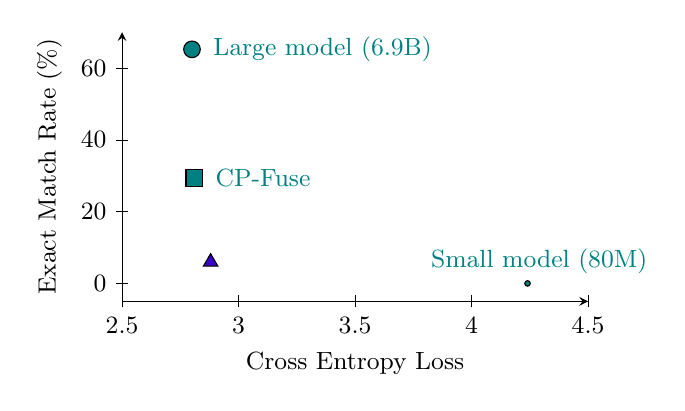
\begin{tikzpicture}
\begin{axis}[
    width=7.5cm,
    height=5cm,
    xlabel=Cross Entropy Loss,
    ylabel=Exact Match Rate (\%),
    xmin=2.5,
    xmax=4.5,
    ymin=-5,
    ymax=70,
    xtick={2.5,3.0,3.5,4.0,4.5},
    ytick={0,20,40,60},
    xlabel near ticks,
    ylabel near ticks,
    axis lines=left,
    clip=false,
    scatter/classes={
        large={mark=*,draw=none,fill=teal},
        small={mark=*,draw=none,fill=teal,mark size=1pt},
        token={mark=triangle*,draw=none,fill=blue!70!purple},
        cpfuse={mark=square*,draw=none,fill=teal}
    },
    tick style={color=black},
    every axis label/.style={font=\small},
    every tick label/.style={font=\small}
]
% Plot points
\addplot[scatter,only marks,
    scatter src=explicit symbolic,
    mark size=3pt]
table[meta=label] {
x    y      label
2.80 65.22  large
4.24 0.00   small
2.88 5.98   token
2.81 29.35  cpfuse
};
% Add labels with nodes
\node[anchor=west, font=\small, text=teal] at (axis cs:2.85,65.22) {Large model (6.9B)};
\node[anchor=south, font=\small, text=teal] at (axis cs:4.29,0.00) {Small model (80M)};
\node[anchor=south, font=\small, text=blue!70!purple] at (axis cs:2.93,5.98) {\sys};
\node[anchor=west, font=\small, text=teal] at (axis cs:2.86,29.35) {CP-Fuse};
\end{axis}
\end{tikzpicture}
\caption{
Comparison of memorization and performance across different model sizes, showing Cross Entropy Loss (CE Loss) versus Exact Match Rate (EMR) (\%). EMR is measured on a subset of Pile~\citep{chang2024localization} and CE Loss on a subset of SlimPajama~\citep{soboleva2023slimpajama}. Larger and more capable models exhibit higher memorization, \sys achieves low memorization rates while maintaining competitive performance. CP-Fuse refers to \citet{abad2024copyright}. More details are given in Section~\ref{subsection:wild}.}
\label{fig:memorizationvsperformance}
\end{figure}


\begin{figure*}[h]
    \label{fig:overview}
    \centering
    \includegraphics[width=\textwidth]{figures/tkswap_pdf.pdf}
    \caption{Overview of \textsc{TokenSwap}. Our approach replaces token probabilities of high-frequency "grammar-based" tokens with those from a small auxiliary language model. This mitigates memorized generation while maintaining fluency and model performance. The top path shows standard LLM generation, while the bottom path demonstrates how \textsc{TokenSwap} alters token selection to disrupt memorization and produce novel text.}
    \label{fig:tkswap_overview}
\end{figure*}

One of the most pressing consequences of memorization is the
reproduction of copyrighted materials. LLMs can generate near-complete
excerpts from their training sets, including literary works, licensed
texts, or proprietary documents \citep{karamolegkou2023copyright}.
This has sparked ongoing legal debates and high-profile lawsuits
aimed at major technology companies for allegedly infringing on
copyrighted content through large-scale AI models
\citep{grynbaum2023times,panwar2025generative}. The issue extends
beyond merely blocking exact substring matches: naive approaches such
as randomly inserting whitespace or special symbols often degrade text
quality and fail to address approximate or near-verbatim copying.
Consequently, users seeking to deploy or integrate LLMs into
production systems require practical methods that effectively disrupt
memorized sequences without sacrificing fluency and semantic accuracy.


Existing approaches to address memorization are broadly categorized into pre-training and post-training interventions. Pre-training methods include deduplication \citep{kandpal2022deduplicating}, differential privacy (DP) \citep{abadi2016deep}, and selective token exclusion during training \citep{hans2024like}. While these approaches can reduce memorization, they often incur substantial computational costs and degrade model performance \citep{Anil2021}. Post-training interventions focus on unlearning techniques that attempt to modify specific neurons and weights \citep{maini2023can, sakarvadia2024mitigating}. However, these methods remain susceptible to training data extraction \citep{shumailov2024ununlearning} and can impair model capabilities \citep{huang2024demystifyingverbatimmemorizationlarge}. This challenge is further complicated by theoretical findings suggesting that some degree of memorization may be inherent to achieving generalization in learning algorithms \citep{attias2024information}.

In contrast, another line of work focuses on preventing the generation of memorized content at inference time. These approaches include blocking exact matches to training data \citep{ippolito2022preventing} or combining logits from multiple models \citep{abad2024copyright}. However, these methods rely on impractical assumptions, such as access to training data or requiring multiple LLMs trained on disjoint datasets.



In this work, we propose \sys, a method that combines probability distributions from large and small language models during generation. While small language models exhibit low memorized generation but poor performance, and large models demonstrate strong capabilities but significant memorization, \sys achieves the best of both worlds: low memorized generation with minimal change in performance (Figure~\ref{fig:memorizationvsperformance}). \sys replaces probabilities of a subset of tokens with those from a smaller language model. Since smaller language models demonstrate significantly lower memorization \citep{carlini2022quantifying, biderman2024emergent}, this effectively disrupts the high-probability pathways that lead to memorized generation. Our theoretical analysis shows that under this approach, the probability of reproducing a memorized sequence relative to its baseline probability decreases exponentially with sequence length (Section~\ref{subsec:theory}).


Unlike prior defenses which require model weights, training data access or multiple large models our approach relies solely on output token probabilities. \textit{This makes our defense uniquely accessible, inexpensive and simple to use.} 


We evaluate \sys through both controlled experiments and real-world deployments. In controlled experiments (Section~\ref{subsection:finetuning}), we create an extreme test case by finetuning models on a small dataset for 50 epochs, where \sys achieves a 50-800x reduction in verbatim generation compared to undefended models. In real-world evaluations (Section~\ref{subsection:wild}), we apply \sys to commercial models including Pythia-6.9b and Llama-3-8b, demonstrating a 10x reduction in verbatim generation while preserving performance on downstream language and commonsense tasks. Our comparisons with Goldfish~\citep{hans2024like}, a pre-training approach for reducing memorization, show that \sys achieves comparable effectiveness, indicating that our post-hoc method can match the performance of pre-training solutions (Section~\ref{subsection:goldfish}).

